% ------------------------------------------------------------------------
% ------------------------------------------------------------------------
% abnTeX2: Modelo de Trabalho Acadêmico em conformidade com 
% as normas da ABNT
% ------------------------------------------------------------------------
% ------------------------------------------------------------------------

\documentclass[english, 
               brazil, 
               bsc] %Opções bsc (TCC) e msc (Mestrado)
               {deagri-abntex2}

% Geração de dummy text
% Retirar para a versão final do documento
\usepackage{lipsum}


%Compila o indice
\makeindex
\usepackage{subfig}
\usepackage{booktabs}
\usepackage{xcolor}

\begin{document}

% Seleciona o idioma do documento (conforme pacotes do babel)
\selectlanguage{brazil}

% Retira espaço extra obsoleto entre as frases.
\frenchspacing 

% ----------------------------------------------------------
% ELEMENTOS PRÉ-TEXTUAIS
% ----------------------------------------------------------
\pretextual

\titulo{Biospeckle em comparação com métodos físico-químicos para análise em tomate}
\autor{Luiz Diego Vidal Santos}
\orientador{Prof. Dr. Adilson Machado Enes}
\coorientador{Prof. Dr. Paulo Roberto Gagliardi}
\curso{Engenharia Agronômica}

\imprimircapa
\imprimirfolhaderosto
\imprimirfolhadeaprovacao
\begin{agradecimentos}

Aos meus pais e irmãs e sobrinhas pelo apoio, colaboração, amor, empenho e paciência.

A minha noiva pelas notes de insonia, todas as revisões realizadas durante todo o curso, pela paciência e companheirismo em todos os mementos de dificuldades.

Ao Professor Dr. Adilson pelos quatro anos de trabalho duro, ensinamento, paciência e presteza no auxílio das atividades e nas discussões sobre os assuntos abordados neste Trabalho de Conclusão de Curso. 

Ao Professor Dr. Paulo Roberto Gagliardi pelos ensinamentos sobre a construção e condução correta deste Trabalho de Conclusão de Curso.
Ao Professor Dr. Luiz Fernando Ganassali de Oliveira Junior pelo espaço cedido e pelos equipamentos laboratoriais do laboratório ECOPOC para que este trabalho fosse realizado.

A todos os professores do DEA pelo carinho, dedicação e entusiasmo demonstrados ao longo do curso. 

Aos colegas de curso especialmente aos companheiros Airton Marques e Igor Sabino pela amizade, companheirismo,  espontaneidade e alegria ao longo de todos esses anos de convivência.

E, finalmente, a Deus pela fé e força depositadas em mim para que eu pudesse enfrentar este curso e conseguir concluí-lo.
\end{agradecimentos}
% ---
\begin{epigrafe}[]
    \vspace*{\fill}
	\begin{flushright}
	
		\textit{Que os vossos esforços desafiem as\\ impossibilidades, lembrai-vos de que as grandes\\ coisas do homem foram conquistadas do que parecia\\ impossível.\\
				\textbf{Charles Chaplin}}
		
	\end{flushright}
\end{epigrafe}
% ---
% resumo em português
\setlength{\absparsep}{18pt} % ajusta o espaçamento dos parágrafos do resumo
\begin{resumo}
 

Lorem ipsum dolor sit amet, consectetur adipiscing elit. Vestibulum sem lectus, vestibulum et semper sit amet, sodales vitae est. Nulla euismod facilisis elementum. Sed non dictum eros, nec malesuada lacus. Praesent ut efficitur mauris. Donec porttitor mattis euismod. Suspendisse tristique lacus lectus, semper dapibus tortor dapibus ac. Donec fermentum leo id erat sagittis porta. Aenean nec pellentesque dui, ac pellentesque diam. Phasellus placerat, augue vitae tincidunt lobortis, risus diam auctor enim, et efficitur nisl dui interdum metus. Nam sapien ligula, porta vitae posuere in, feugiat at massa. In vel sodales enim. Phasellus volutpat condimentum quam, sed ultrices velit. Duis malesuada tincidunt tempus. Aliquam lectus purus, semper quis ante in, rhoncus convallis quam. Maecenas ex neque, aliquet sit amet lobortis vitae, blandit quis purus. Aliquam aliquam quam vel rhoncus placerat. Duis nulla neque, euismod ac pharetra non, tempor eu quam. Nulla sollicitudin, risus in vestibulum ullamcorper, dolor justo suscipit nisl, at luctus nunc ex eget neque. Maecenas quis felis sapien. Vivamus tempor et neque sit amet dignissim. Aliquam pulvinar turpis in tortor ultrices ornare. Etiam ultricies vel sapien vitae gravida. Donec lorem velit, commodo in convallis eu, tristique eu dui. Donec bibendum leo mi, non consequat arcu aliquet ut. Ut consectetur lacus eros, nec efficitur sem faucibus a. Donec sit amet nulla facilisis, euismod libero eget, auctor nisl. Pellentesque habitant morbi tristique senectus et netus et malesuada fames ac turpis egestas. Vestibulum vitae massa quis ante malesuada tristique. Praesent posuere enim non urna convallis hendrerit. Vestibulum neque ligula, varius quis vehicula ut, lacinia vitae eros. Curabitur at lectus sagittis, tempus nunc ac, maximus massa. Pellentesque vehicula, eros tincidunt accumsan ultricies, elit diam cursus leo, eget dapibus sem orci non neque. Vivamus auctor erat ac metus imperdiet, ut sagittis justo dapibus.
 \\

 \textbf{Palavras-chave}: Fruto hortícola, Laser HeNe, \emph{Solanum Lycopersicum}, Processamento de Sinais.
\end{resumo}
% resumo em inglês
\setlength{\absparsep}{18pt} % ajusta o espaçamento dos parágrafos do resumo
\begin{resumo}[Abstract]
 \begin{otherlanguage*}{english}
   
Lorem ipsum dolor sit amet, consectetur adipiscing elit. Vestibulum sem lectus, vestibulum et semper sit amet, sodales vitae est. Nulla euismod facilisis elementum. Sed non dictum eros, nec malesuada lacus. Praesent ut efficitur mauris. Donec porttitor mattis euismod. Suspendisse tristique lacus lectus, semper dapibus tortor dapibus ac. Donec fermentum leo id erat sagittis porta. Aenean nec pellentesque dui, ac pellentesque diam. Phasellus placerat, augue vitae tincidunt lobortis, risus diam auctor enim, et efficitur nisl dui interdum metus. Nam sapien ligula, porta vitae posuere in, feugiat at massa. In vel sodales enim. Phasellus volutpat condimentum quam, sed ultrices velit. Duis malesuada tincidunt tempus. Aliquam lectus purus, semper quis ante in, rhoncus convallis quam. Maecenas ex neque, aliquet sit amet lobortis vitae, blandit quis purus. Aliquam aliquam quam vel rhoncus placerat. Duis nulla neque, euismod ac pharetra non, tempor eu quam. Nulla sollicitudin, risus in vestibulum ullamcorper, dolor justo suscipit nisl, at luctus nunc ex eget neque. Maecenas quis felis sapien. Vivamus tempor et neque sit amet dignissim. Aliquam pulvinar turpis in tortor ultrices ornare. Etiam ultricies vel sapien vitae gravida. Donec lorem velit, commodo in convallis eu, tristique eu dui. Donec bibendum leo mi, non consequat arcu aliquet ut. Ut consectetur lacus eros, nec efficitur sem faucibus a. Donec sit amet nulla facilisis, euismod libero eget, auctor nisl. Pellentesque habitant morbi tristique senectus et netus et malesuada fames ac turpis egestas. Vestibulum vitae massa quis ante malesuada tristique. Praesent posuere enim non urna convallis hendrerit. Vestibulum neque ligula, varius quis vehicula ut, lacinia vitae eros. Curabitur at lectus sagittis, tempus nunc ac, maximus massa. Pellentesque vehicula, eros tincidunt accumsan ultricies, elit diam cursus leo, eget dapibus sem orci non neque. Vivamus auctor erat ac metus imperdiet, ut sagittis justo dapibus.


 \textbf{Keywords}: Horticultural fruit, HeNe Laser, \emph{Solanum lycopersicum}, Signal Processing.
 \end{otherlanguage*}
\end{resumo}

% Pacote para a definição de novas cores
 
% Lista de Figuras
\pdfbookmark[0]{\listfigurename}{lof}
\listoffigures*
\cleardoublepage

 %Lista de Tabelas
\pdfbookmark[0]{\listtablename}{lot}
\listoftables*
\cleardoublepage

% Lista de Códigos
\pdfbookmark[0]{\listlistingname}{lol}
\begin{KeepFromToc}
	\listoflistings
\end{KeepFromToc}
\cleardoublepage

% ---
% inserir lista de abreviaturas e siglas
% ---

\begin{siglas}
  	\item[COM]{Concurrence Matrix}
  	\item[DG]{Diferença Generaliazada}
  	\item[FFT]{Fast Fourier Transforme}
	\item[MI]{Momento de Inércia}
	\item[MOC]{Matriz de Ocorrência Modificada}
	\item[PME]{Pectina Metil Esterase}
	\item[PDI]{Processamento Digital de Imagens}
	\item[STS]{Padrão Temporal do Speckle}
	\item[TF]{Trasnformada de Fourier}
	\item[TFJ]{Trasnformada de Fourier Janelada}
\end{siglas}
% ---
% ---
% inserir lista de símbolos
% ---

\begin{simbolos}
  \item[$ \sum  $] Letra grega Sigma
  \item[$ \int $] Integral
  \item[$ \omega $] Letra grega ómega
\end{simbolos}
% ---
    
\pdfbookmark[0]{\contentsname}{toc}
\tableofcontents*

% ----------------------------------------------------------
% ELEMENTOS TEXTUAIS
% ----------------------------------------------------------
\textual
\newpage

\chapter{Introdução}

Lorem ipsum dolor sit amet, consectetur adipiscing elit. Vestibulum sem lectus, vestibulum et semper sit amet, sodales vitae est. Nulla euismod facilisis elementum. Sed non dictum eros, nec malesuada lacus. Praesent ut efficitur mauris. Donec porttitor mattis euismod. Suspendisse tristique lacus lectus, semper dapibus tortor dapibus ac. Donec fermentum leo id erat sagittis porta. Aenean nec pellentesque dui, ac pellentesque diam. Phasellus placerat, augue vitae tincidunt lobortis, risus diam auctor enim, et efficitur nisl dui interdum metus. Nam sapien ligula, porta vitae posuere in, feugiat at massa. In vel sodales enim.

Phasellus volutpat condimentum quam, sed ultrices velit. Duis malesuada tincidunt tempus. Aliquam lectus purus, semper quis ante in, rhoncus convallis quam. Maecenas ex neque, aliquet sit amet lobortis vitae, blandit quis purus. Aliquam aliquam quam vel rhoncus placerat. Duis nulla neque, euismod ac pharetra non, tempor eu quam. Nulla sollicitudin, risus in vestibulum ullamcorper, dolor justo suscipit nisl, at luctus nunc ex eget neque. Maecenas quis felis sapien. Vivamus tempor et neque sit amet dignissim. Aliquam pulvinar turpis in tortor ultrices ornare. Etiam ultricies vel sapien vitae gravida.

Donec lorem velit, commodo in convallis eu, tristique eu dui. Donec bibendum leo mi, non consequat arcu aliquet ut. Ut consectetur lacus eros, nec efficitur sem faucibus a. Donec sit amet nulla facilisis, euismod libero eget, auctor nisl. Pellentesque habitant morbi tristique senectus et netus et malesuada fames ac turpis egestas. Vestibulum vitae massa quis ante malesuada tristique. Praesent posuere enim non urna convallis hendrerit. Vestibulum neque ligula, varius quis vehicula ut, lacinia vitae eros. Curabitur at lectus sagittis, tempus nunc ac, maximus massa. Pellentesque vehicula, eros tincidunt accumsan ultricies, elit diam cursus leo, eget dapibus sem orci non neque. Vivamus auctor erat ac metus imperdiet, ut sagittis justo dapibus.

Ut dapibus elit sed elementum maximus. Praesent maximus convallis lacus, vitae tempor purus euismod et. Donec elementum id dui vel aliquet. Maecenas at convallis est, at faucibus nisi. Aliquam quis euismod lorem. Vivamus in ex a diam vehicula finibus. Sed venenatis vitae risus eget fermentum. Nunc ullamcorper neque id dolor porta, in fringilla diam lobortis.

Cras vehicula venenatis augue, et venenatis eros feugiat sit amet. Duis tellus urna, eleifend quis erat sed, elementum euismod elit. Donec vel ex luctus, porttitor erat sit amet, malesuada lectus. Cras at nisi ligula. Vestibulum sit amet ullamcorper tortor. Suspendisse potenti. Nam vehicula turpis ante, id aliquet ante varius non.

\section{Tema}
Uso do Biospeckle dinâmico laser na análise da qualidade do tomate Caline IPA-6 no período de 15 dias pós-colheita.
%\emph{abntex2} comando para deixar letras em itálico



\section{Problema}


Lorem ipsum dolor sit amet, consectetur adipiscing elit. Vestibulum sem lectus, vestibulum et semper sit amet, sodales vitae est. Nulla euismod facilisis elementum. Sed non dictum eros, nec malesuada lacus. Praesent ut efficitur mauris. Donec porttitor mattis euismod. Suspendisse tristique lacus lectus, semper dapibus tortor dapibus ac. Donec fermentum leo id erat sagittis porta. Aenean nec pellentesque dui, ac pellentesque diam. Phasellus placerat, augue vitae tincidunt lobortis, risus diam auctor enim, et efficitur nisl dui interdum metus. Nam sapien ligula, porta vitae posuere in, feugiat at massa. In vel sodales enim.

\section{Hipótese}


Lorem ipsum dolor sit amet, consectetur adipiscing elit. Vestibulum sem lectus, vestibulum et semper sit amet, sodales vitae est. Nulla euismod facilisis elementum. Sed non dictum eros, nec malesuada lacus. Praesent ut efficitur mauris. Donec porttitor mattis euismod.

\section{Objetivo}
\begin{itemize}

\item { Suspendisse tristique lacus lectus, semper dapibus tortor dapibus ac. Donec fermentum leo id erat sagittis porta. Aenean nec pellentesque dui, ac pellentesque diam. Phasellus placerat, augue vitae tincidunt lobortis, risus diam auctor enim, et efficitur nisl dui interdum metus. Nam sapien ligula, porta vitae posuere in, feugiat at massa. In vel sodales enim.} 
\end{itemize}

\subsection{Objetivos Específicos}

\begin{itemize}
\item {Phasellus volutpat condimentum quam, sed ultrices velit. Duis malesuada tincidunt tempus;}
\item{Phasellus volutpat condimentum quam, sed ultrices velit. Duis malesuada tincidunt tempus. }
\item {Phasellus volutpat condimentum quam, sed ultrices velit. Duis malesuada tincidunt tempus. }
\end{itemize}

\section{Justificativa}
Lorem ipsum dolor sit amet, consectetur adipiscing elit. Vestibulum sem lectus, vestibulum et semper sit amet, sodales vitae est. Nulla euismod facilisis elementum. Sed non dictum eros, nec malesuada lacus. Praesent ut efficitur mauris. Donec porttitor mattis euismod. Suspendisse tristique lacus lectus, semper dapibus tortor dapibus ac. Donec fermentum leo id erat sagittis porta. Aenean nec pellentesque dui, ac pellentesque diam. Phasellus placerat, augue vitae tincidunt lobortis, risus diam auctor enim, et efficitur nisl dui interdum metus. Nam sapien ligula, porta vitae posuere in, feugiat at massa. In vel sodales enim.

Phasellus volutpat condimentum quam, sed ultrices velit. Duis malesuada tincidunt tempus. Aliquam lectus purus, semper quis ante in, rhoncus convallis quam. Maecenas ex neque, aliquet sit amet lobortis vitae, blandit quis purus. Aliquam aliquam quam vel rhoncus placerat. Duis nulla neque, euismod ac pharetra non, tempor eu quam. Nulla sollicitudin, risus in vestibulum ullamcorper, dolor justo suscipit nisl, at luctus nunc ex eget neque. Maecenas quis felis sapien. Vivamus tempor et neque sit amet dignissim. Aliquam pulvinar turpis in tortor ultrices ornare. Etiam ultricies vel sapien vitae gravida.

Donec lorem velit, commodo in convallis eu, tristique eu dui. Donec bibendum leo mi, non consequat arcu aliquet ut. Ut consectetur lacus eros, nec efficitur sem faucibus a. Donec sit amet nulla facilisis, euismod libero eget, auctor nisl. Pellentesque habitant morbi tristique senectus et netus et malesuada fames ac turpis egestas. Vestibulum vitae massa quis ante malesuada tristique. Praesent posuere enim non urna convallis hendrerit. Vestibulum neque ligula, varius quis vehicula ut, lacinia vitae eros. Curabitur at lectus sagittis, tempus nunc ac, maximus massa. Pellentesque vehicula, eros tincidunt accumsan ultricies, elit diam cursus leo, eget dapibus sem orci non neque. Vivamus auctor erat ac metus imperdiet, ut sagittis justo dapibus.


\chapter{Revisão de literatura}

\section{\emph{Solanum Lycopersicum L.}}
Lorem ipsum dolor sit amet, consectetur adipiscing elit. Vestibulum sem lectus, vestibulum et semper sit amet, sodales vitae est. Nulla euismod facilisis elementum. Sed non dictum eros, nec malesuada lacus. Praesent ut efficitur mauris. Donec porttitor mattis euismod. Suspendisse tristique lacus lectus, semper dapibus tortor dapibus ac. Donec fermentum leo id erat sagittis porta. Aenean nec pellentesque dui, ac pellentesque diam. Phasellus placerat, augue vitae tincidunt lobortis, risus diam auctor enim, et efficitur nisl dui interdum metus. Nam sapien ligula, porta vitae posuere in, feugiat at massa. In vel sodales enim.

Phasellus volutpat condimentum quam, sed ultrices velit. Duis malesuada tincidunt tempus. Aliquam lectus purus, semper quis ante in, rhoncus convallis quam. Maecenas ex neque, aliquet sit amet lobortis vitae, blandit quis purus. Aliquam aliquam quam vel rhoncus placerat. Duis nulla neque, euismod ac pharetra non, tempor eu quam. Nulla sollicitudin, risus in vestibulum ullamcorper, dolor justo suscipit nisl, at luctus nunc ex eget neque. Maecenas quis felis sapien. Vivamus tempor et neque sit amet dignissim. Aliquam pulvinar turpis in tortor ultrices ornare. Etiam ultricies vel sapien vitae gravida.

Donec lorem velit, commodo in convallis eu, tristique eu dui. Donec bibendum leo mi, non consequat arcu aliquet ut. Ut consectetur lacus eros, nec efficitur sem faucibus a. Donec sit amet nulla facilisis, euismod libero eget, auctor nisl. Pellentesque habitant morbi tristique senectus et netus et malesuada fames ac turpis egestas. Vestibulum vitae massa quis ante malesuada tristique. Praesent posuere enim non urna convallis hendrerit. Vestibulum neque ligula, varius quis vehicula ut, lacinia vitae eros. Curabitur at lectus sagittis, tempus nunc ac, maximus massa. Pellentesque vehicula, eros tincidunt accumsan ultricies, elit diam cursus leo, eget dapibus sem orci non neque. Vivamus auctor erat ac metus imperdiet, ut sagittis justo dapibus.

Ut dapibus elit sed elementum maximus. Praesent maximus convallis lacus, vitae tempor purus euismod et. Donec elementum id dui vel aliquet. Maecenas at convallis est, at faucibus nisi. Aliquam quis euismod lorem. Vivamus in ex a diam vehicula finibus. Sed venenatis vitae risus eget fermentum. Nunc ullamcorper neque id dolor porta, in fringilla diam lobortis.

Cras vehicula venenatis augue, et venenatis eros feugiat sit amet. Duis tellus urna, eleifend quis erat sed, elementum euismod elit. Donec vel ex luctus, porttitor erat sit amet, malesuada lectus. Cras at nisi ligula. Vestibulum sit amet ullamcorper tortor. Suspendisse potenti. Nam vehicula turpis ante, id aliquet ante varius non.


\section{Considerações iniciais sobre o Biospeckle}

%%%%%%%%%%%%%%%%%%%%%%%%%%%%%%% exemplo de Figúra%%%%%%%%%%%%%%%%

\begin{figure}[!htb]
	\caption{Imagens de STS sem atividade e com alta atividade respectivamente.
}
  \centering
  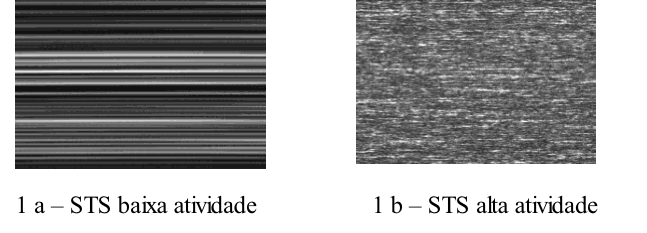
\includegraphics[scale=1.0]{Imagens/imagem_1.png} 
  \legend{Fonte: \cite{enes_alise_2006}}
  \label{figura0}
\end{figure}

% %Com o newpage vou forçar a descrição ficar na próxima página
Lorem ipsum dolor sit amet, consectetur adipiscing elit. Vestibulum sem lectus, vestibulum et semper sit amet, sodales vitae est. Nulla euismod facilisis elementum. Sed non dictum eros, nec malesuada lacus. Praesent ut efficitur mauris. Donec porttitor mattis euismod. Suspendisse tristique lacus lectus, semper dapibus tortor dapibus ac. Donec fermentum leo id erat sagittis porta. Aenean nec pellentesque dui, ac pellentesque diam. Phasellus placerat, augue vitae tincidunt lobortis, risus diam auctor enim, et efficitur nisl dui interdum metus. Nam sapien ligula, porta vitae posuere in, feugiat at massa. In vel sodales enim.



%%%%%%%%%%%%%%%%%%%%%%%%% Equação%%%%%%%%%%%%%%%%
\begin{equation} \label{eq:01}
CON = \left | Nij \right |
\end{equation}


em que,

\textbf{Nij} – número de ocorrências de intensidades
\textbf{i,j} – intensidades sucessivas

Lorem ipsum dolor sit amet, consectetur adipiscing elit. Vestibulum sem lectus, vestibulum et semper sit amet, sodales vitae est. Nulla euismod facilisis elementum. Sed non dictum eros, nec malesuada lacus. Praesent ut efficitur mauris. Donec porttitor mattis euismod. Suspendisse tristique lacus lectus, semper dapibus tortor dapibus ac. Donec fermentum leo id erat sagittis porta. Aenean nec pellentesque dui, ac pellentesque diam. Phasellus placerat, augue vitae tincidunt lobortis, risus diam auctor enim, et efficitur nisl dui interdum metus. Nam sapien ligula, porta vitae posuere in, feugiat at massa. In vel sodales enim.Lorem ipsum dolor sit amet, consectetur adipiscing elit. Vestibulum sem lectus, vestibulum et semper sit amet, sodales vitae est. Nulla euismod facilisis elementum. Sed non dictum eros, nec malesuada lacus. Praesent ut efficitur mauris. Donec porttitor mattis euismod. Suspendisse tristique lacus lectus, semper dapibus tortor dapibus ac. Donec fermentum leo id erat sagittis porta. Aenean nec pellentesque dui, ac pellentesque diam. Phasellus placerat, augue vitae tincidunt lobortis, risus diam auctor enim, et efficitur nisl dui interdum metus. Nam sapien ligula, porta vitae posuere in, feugiat at massa. In vel sodales enim.

\begin{equation} \label{eq:02}
MDI = \sum_{ij} M ij(i-j)^{2}
\end{equation}

\section{Análise de frequência do Biospeckle laser}


\subsection{A transformada de Fourier}

Lorem ipsum dolor sit amet, consectetur adipiscing elit. Vestibulum sem lectus, vestibulum et semper sit amet, sodales vitae est. Nulla euismod facilisis elementum. Sed non dictum eros, nec malesuada lacus. Praesent ut efficitur mauris. Donec porttitor mattis euismod. Suspendisse tristique lacus lectus, semper dapibus tortor dapibus ac. Donec fermentum leo id erat sagittis porta. Aenean nec pellentesque dui, ac pellentesque diam. Phasellus placerat, augue vitae tincidunt lobortis, risus diam auctor enim, et efficitur nisl dui interdum metus. Nam sapien ligula, porta vitae posuere in, feugiat at massa. In vel sodales enim.

\begin{equation} \label{eq:03}
F(w)=\int_{-\infty }^{\infty} f(t)e^{-wt} dt
\end{equation}



%%%%%%%%%%%%%%% Exemplo de código%%%%%%%%%%
\begin{listing}[H]
    \caption{Trecho código para divisão em Frames}
    \label{labelFrame}
	\begin{minted}{MATLAB}
    for img = 1:128;
    filename=strcat('seed',num2str(img),'.bmp'); 
    frame2 = read(a, img);
    img2 = uint8(frame2(1:480,1:640));
    imwrite(img2,filename);
	\end{minted}
	\label{cod2}

\end{listing}



\chapter{Resultados}

\section{Resultados da análise dos estádios de maturação}
Lorem ipsum dolor sit amet, consectetur adipiscing elit. Vestibulum sem lectus, vestibulum et semper sit amet, sodales vitae est. Nulla euismod facilisis elementum. Sed non dictum eros, nec malesuada lacus. Praesent ut efficitur mauris. Donec porttitor mattis euismod. Suspendisse tristique lacus lectus, semper dapibus tortor dapibus ac. Donec fermentum leo id erat sagittis porta. Aenean nec pellentesque dui, ac pellentesque diam. Phasellus placerat, augue vitae tincidunt lobortis, risus diam auctor enim, et efficitur nisl dui interdum metus. Nam sapien ligula, porta vitae posuere in, feugiat at massa. In vel sodales enim.

Phasellus volutpat condimentum quam, sed ultrices velit. Duis malesuada tincidunt tempus. Aliquam lectus purus, semper quis ante in, rhoncus convallis quam. Maecenas ex neque, aliquet sit amet lobortis vitae, blandit quis purus. Aliquam aliquam quam vel rhoncus placerat. Duis nulla neque, euismod ac pharetra non, tempor eu quam. Nulla sollicitudin, risus in vestibulum ullamcorper, dolor justo suscipit nisl, at luctus nunc ex eget neque. Maecenas quis felis sapien. Vivamus tempor et neque sit amet dignissim. Aliquam pulvinar turpis in tortor ultrices ornare. Etiam ultricies vel sapien vitae gravida.
.

\noindent
\begin{table}[!htb]
\centering
\begin{tabular}{@{}lllllllll@{}}
\toprule
\multicolumn{9}{c}{\textbf{Métodos Físico e Químicos}}                                    \\ \midrule
Tratamento      & TSS     & AT   & COMP (mm) & PMF(g) & FIR(N) & MI     & DI (mm) & pH    \\ \midrule
\textbf{Dia 0}  & 3,74a   & 2,5a & 64,098a   & 0,00d  & 23,56a & 18a    & 45,888b & 4,67a \\ \midrule
\textbf{Dia 3}  & 4,02abc & 3,4a & 68,538a   & 3,8c   & 23,56a & 16,3ab & 48,882b & 4,44a \\ \midrule
\textbf{Dia 6}  & 4,48a & 2,64a & 66,102a &	5,92b &	24,09a & 17,3a & 52,102b & 4,59a \\ \midrule
\textbf{Dia 9}   & 3,88bc & 2,08a & 50,038b & 8,16a & 21,69a & 7,6ab & 67,15a & 4,74a \\ \midrule
\textbf{Dia 12}  & 4,44ab & 2,18a & 70,562a & 9,94a & 19,30a & 5,8b & 46,046b & 4,62a \\ \bottomrule
\end{tabular}
\caption{Valores médios e diferença significativa a 5\% de (TSS) Total Sólidos Solúveis, (AT) Acidez Titulável, (COMP) Comprimento, (PMF) Perda de Massa Fresca, (FIR) Firmeza, (MI) Momento de Inércia, (DI) Diâmetro e (pH)}
\label{tab1}
\end{table}



\clearpage


\chapter{Conclusão}

Lorem ipsum dolor sit amet, consectetur adipiscing elit. Vestibulum sem lectus, vestibulum et semper sit amet, sodales vitae est. Nulla euismod facilisis elementum. Sed non dictum eros, nec malesuada lacus. Praesent ut efficitur mauris. Donec porttitor mattis euismod. Suspendisse tristique lacus lectus, semper dapibus tortor dapibus ac. Donec fermentum leo id erat sagittis porta. Aenean nec pellentesque dui, ac pellentesque diam. Phasellus placerat, augue vitae tincidunt lobortis, risus diam auctor enim, et efficitur nisl dui interdum metus. Nam sapien ligula, porta vitae posuere in, feugiat at massa. In vel sodales enim.

Phasellus volutpat condimentum quam, sed ultrices velit. Duis malesuada tincidunt tempus. Aliquam lectus purus, semper quis ante in, rhoncus convallis quam. Maecenas ex neque, aliquet sit amet lobortis vitae, blandit quis purus. Aliquam aliquam quam vel rhoncus placerat. Duis nulla neque, euismod ac pharetra non, tempor eu quam. Nulla sollicitudin, risus in vestibulum ullamcorper, dolor justo suscipit nisl, at luctus nunc ex eget neque. Maecenas quis felis sapien. Vivamus tempor et neque sit amet dignissim. Aliquam pulvinar turpis in tortor ultrices ornare. Etiam ultricies vel sapien vitae gravida.




% ----------------------------------------------------------
% ELEMENTOS PÓS-TEXTUAIS
% ----------------------------------------------------------
\postextual
\bibliography{references} %erro no zotero, verificar com mendeley

\renewcommand{\chapnumfont}{\chaptitlefont}
\renewcommand{\afterchapternum}{}
%\begin{apendicesenv}

% Imprime uma página indicando o início dos apêndices
\partapendices

% ----------------------------------------------------------
\chapter{Quisque libero justo}
% ----------------------------------------------------------

\lipsum[50]

% ----------------------------------------------------------
\chapter{Nullam elementum urna vel imperdiet sodales elit ipsum pharetra ligula
ac pretium ante justo a nulla curabitur tristique arcu eu metus}
% ----------------------------------------------------------
\lipsum[55-57]

\end{apendicesenv}

%\begin{anexosenv}


% Imprime uma página indicando o início dos anexos
\partanexos

% ---
\chapter{Morbi ultrices rutrum lorem.}
% ---
\lipsum[30]

% ---
\chapter{Cras non urna sed feugiat cum sociis natoque penatibus et magnis dis
parturient montes nascetur ridiculus mus}
% ---

\lipsum[31]

% ---
\chapter{Fusce facilisis lacinia dui}
% ---

\lipsum[32]


\end{anexosenv}


\end{document}